%% bare_conf.tex
%% V1.4b
%% 2015/08/26
%% by Michael Shell
%% See:
%% http://www.michaelshell.org/
%% for current contact information.
%%
%% This is a skeleton file demonstrating the use of IEEEtran.cls
%% (requires IEEEtran.cls version 1.8b or later) with an IEEE
%% conference paper.
%%
%% Support sites:
%% http://www.michaelshell.org/tex/ieeetran/
%% http://www.ctan.org/pkg/ieeetran
%% and
%% http://www.ieee.org/

%%*************************************************************************
%% Legal Notice:
%% This code is offered as-is without any warranty either expressed or
%% implied; without even the implied warranty of MERCHANTABILITY or
%% FITNESS FOR A PARTICULAR PURPOSE! 
%% User assumes all risk.
%% In no event shall the IEEE or any contributor to this code be liable for
%% any damages or losses, including, but not limited to, incidental,
%% consequential, or any other damages, resulting from the use or misuse
%% of any information contained here.
%%
%% All comments are the opinions of their respective authors and are not
%% necessarily endorsed by the IEEE.
%%
%% This work is distributed under the LaTeX Project Public License (LPPL)
%% ( http://www.latex-project.org/ ) version 1.3, and may be freely used,
%% distributed and modified. A copy of the LPPL, version 1.3, is included
%% in the base LaTeX documentation of all distributions of LaTeX released
%% 2003/12/01 or later.
%% Retain all contribution notices and credits.
%% ** Modified files should be clearly indicated as such, including  **
%% ** renaming them and changing author support contact information. **
%%*************************************************************************


% *** Authors should verify (and, if needed, correct) their LaTeX system  ***
% *** with the testflow diagnostic prior to trusting their LaTeX platform ***
% *** with production work. The IEEE's font choices and paper sizes can   ***
% *** trigger bugs that do not appear when using other class files.       ***                          ***
% The testflow support page is at:
% http://www.michaelshell.org/tex/testflow/


\documentclass[conference]{IEEEtran}
\usepackage{titlesec}
\usepackage{url}
\makeatletter
\newcommand*{\rom}[1]{\expandafter\@slowromancap\romannumeral #1@}
\makeatother
\usepackage{amsmath}
\usepackage{amssymb}
\DeclareMathOperator*{\argmax}{arg\,max}
\DeclareMathOperator*{\argmin}{arg\,min}
\DeclareMathOperator{\EX}{\mathbb{E}}
\usepackage{graphicx}
\usepackage{float}
\usepackage[section]{placeins}
% Some Computer Society conferences also require the compsoc mode option,
% but others use the standard conference format.
%
% If IEEEtran.cls has not been installed into the LaTeX system files,
% manually specify the path to it like:
% \documentclass[conference]{../sty/IEEEtran}





% Some very useful LaTeX packages include:
% (uncomment the ones you want to load)


% *** MISC UTILITY PACKAGES ***
%
%\usepackage{ifpdf}
% Heiko Oberdiek's ifpdf.sty is very useful if you need conditional
% compilation based on whether the output is pdf or dvi.
% usage:
% \ifpdf
%   % pdf code
% \else
%   % dvi code
% \fi
% The latest version of ifpdf.sty can be obtained from:
% http://www.ctan.org/pkg/ifpdf
% Also, note that IEEEtran.cls V1.7 and later provides a builtin
% \ifCLASSINFOpdf conditional that works the same way.
% When switching from latex to pdflatex and vice-versa, the compiler may
% have to be run twice to clear warning/error messages.






% *** CITATION PACKAGES ***
%
%\usepackage{cite}
% cite.sty was written by Donald Arseneau
% V1.6 and later of IEEEtran pre-defines the format of the cite.sty package
% \cite{} output to follow that of the IEEE. Loading the cite package will
% result in citation numbers being automatically sorted and properly
% "compressed/ranged". e.g., [1], [9], [2], [7], [5], [6] without using
% cite.sty will become [1], [2], [5]--[7], [9] using cite.sty. cite.sty's
% \cite will automatically add leading space, if needed. Use cite.sty's
% noadjust option (cite.sty V3.8 and later) if you want to turn this off
% such as if a citation ever needs to be enclosed in parenthesis.
% cite.sty is already installed on most LaTeX systems. Be sure and use
% version 5.0 (2009-03-20) and later if using hyperref.sty.
% The latest version can be obtained at:
% http://www.ctan.org/pkg/cite
% The documentation is contained in the cite.sty file itself.






% *** GRAPHICS RELATED PACKAGES ***
%
\ifCLASSINFOpdf
% \usepackage[pdftex]{graphicx}
% declare the path(s) where your graphic files are
% \graphicspath{{../pdf/}{../jpeg/}}
% and their extensions so you won't have to specify these with
% every instance of \includegraphics
% \DeclareGraphicsExtensions{.pdf,.jpeg,.png}
\else
% or other class option (dvipsone, dvipdf, if not using dvips). graphicx
% will default to the driver specified in the system graphics.cfg if no
% driver is specified.
% \usepackage[dvips]{graphicx}
% declare the path(s) where your graphic files are
% \graphicspath{{../eps/}}
% and their extensions so you won't have to specify these with
% every instance of \includegraphics
% \DeclareGraphicsExtensions{.eps}
\fi
% graphicx was written by David Carlisle and Sebastian Rahtz. It is
% required if you want graphics, photos, etc. graphicx.sty is already
% installed on most LaTeX systems. The latest version and documentation
% can be obtained at: 
% http://www.ctan.org/pkg/graphicx
% Another good source of documentation is "Using Imported Graphics in
% LaTeX2e" by Keith Reckdahl which can be found at:
% http://www.ctan.org/pkg/epslatex
%
% latex, and pdflatex in dvi mode, support graphics in encapsulated
% postscript (.eps) format. pdflatex in pdf mode supports graphics
% in .pdf, .jpeg, .png and .mps (metapost) formats. Users should ensure
% that all non-photo figures use a vector format (.eps, .pdf, .mps) and
% not a bitmapped formats (.jpeg, .png). The IEEE frowns on bitmapped formats
% which can result in "jaggedy"/blurry rendering of lines and letters as
% well as large increases in file sizes.
%
% You can find documentation about the pdfTeX application at:
% http://www.tug.org/applications/pdftex





% *** MATH PACKAGES ***
%
%\usepackage{amsmath}
% A popular package from the American Mathematical Society that provides
% many useful and powerful commands for dealing with mathematics.
%
% Note that the amsmath package sets \interdisplaylinepenalty to 10000
% thus preventing page breaks from occurring within multiline equations. Use:
%\interdisplaylinepenalty=2500
% after loading amsmath to restore such page breaks as IEEEtran.cls normally
% does. amsmath.sty is already installed on most LaTeX systems. The latest
% version and documentation can be obtained at:
% http://www.ctan.org/pkg/amsmath





% *** SPECIALIZED LIST PACKAGES ***
%
%\usepackage{algorithmic}
% algorithmic.sty was written by Peter Williams and Rogerio Brito.
% This package provides an algorithmic environment fo describing algorithms.
% You can use the algorithmic environment in-text or within a figure
% environment to provide for a floating algorithm. Do NOT use the algorithm
% floating environment provided by algorithm.sty (by the same authors) or
% algorithm2e.sty (by Christophe Fiorio) as the IEEE does not use dedicated
% algorithm float types and packages that provide these will not provide
% correct IEEE style captions. The latest version and documentation of
% algorithmic.sty can be obtained at:
% http://www.ctan.org/pkg/algorithms
% Also of interest may be the (relatively newer and more customizable)
% algorithmicx.sty package by Szasz Janos:
% http://www.ctan.org/pkg/algorithmicx




% *** ALIGNMENT PACKAGES ***
%
%\usepackage{array}
% Frank Mittelbach's and David Carlisle's array.sty patches and improves
% the standard LaTeX2e array and tabular environments to provide better
% appearance and additional user controls. As the default LaTeX2e table
% generation code is lacking to the point of almost being broken with
% respect to the quality of the end results, all users are strongly
% advised to use an enhanced (at the very least that provided by array.sty)
% set of table tools. array.sty is already installed on most systems. The
% latest version and documentation can be obtained at:
% http://www.ctan.org/pkg/array


% IEEEtran contains the IEEEeqnarray family of commands that can be used to
% generate multiline equations as well as matrices, tables, etc., of high
% quality.




% *** SUBFIGURE PACKAGES ***
%\ifCLASSOPTIONcompsoc
%  \usepackage[caption=false,font=normalsize,labelfont=sf,textfont=sf]{subfig}
%\else
%  \usepackage[caption=false,font=footnotesize]{subfig}
%\fi
% subfig.sty, written by Steven Douglas Cochran, is the modern replacement
% for subfigure.sty, the latter of which is no longer maintained and is
% incompatible with some LaTeX packages including fixltx2e. However,
% subfig.sty requires and automatically loads Axel Sommerfeldt's caption.sty
% which will override IEEEtran.cls' handling of captions and this will result
% in non-IEEE style figure/table captions. To prevent this problem, be sure
% and invoke subfig.sty's "caption=false" package option (available since
% subfig.sty version 1.3, 2005/06/28) as this is will preserve IEEEtran.cls
% handling of captions.
% Note that the Computer Society format requires a larger sans serif font
% than the serif footnote size font used in traditional IEEE formatting
% and thus the need to invoke different subfig.sty package options depending
% on whether compsoc mode has been enabled.
%
% The latest version and documentation of subfig.sty can be obtained at:
% http://www.ctan.org/pkg/subfig




% *** FLOAT PACKAGES ***
%
%\usepackage{fixltx2e}
% fixltx2e, the successor to the earlier fix2col.sty, was written by
% Frank Mittelbach and David Carlisle. This package corrects a few problems
% in the LaTeX2e kernel, the most notable of which is that in current
% LaTeX2e releases, the ordering of single and double column floats is not
% guaranteed to be preserved. Thus, an unpatched LaTeX2e can allow a
% single column figure to be placed prior to an earlier double column
% figure.
% Be aware that LaTeX2e kernels dated 2015 and later have fixltx2e.sty's
% corrections already built into the system in which case a warning will
% be issued if an attempt is made to load fixltx2e.sty as it is no longer
% needed.
% The latest version and documentation can be found at:
% http://www.ctan.org/pkg/fixltx2e


%\usepackage{stfloats}
% stfloats.sty was written by Sigitas Tolusis. This package gives LaTeX2e
% the ability to do double column floats at the bottom of the page as well
% as the top. (e.g., "\begin{figure*}[!b]" is not normally possible in
% LaTeX2e). It also provides a command:
%\fnbelowfloat
% to enable the placement of footnotes below bottom floats (the standard
% LaTeX2e kernel puts them above bottom floats). This is an invasive package
% which rewrites many portions of the LaTeX2e float routines. It may not work
% with other packages that modify the LaTeX2e float routines. The latest
% version and documentation can be obtained at:
% http://www.ctan.org/pkg/stfloats
% Do not use the stfloats baselinefloat ability as the IEEE does not allow
% \baselineskip to stretch. Authors submitting work to the IEEE should note
% that the IEEE rarely uses double column equations and that authors should try
% to avoid such use. Do not be tempted to use the cuted.sty or midfloat.sty
% packages (also by Sigitas Tolusis) as the IEEE does not format its papers in
% such ways.
% Do not attempt to use stfloats with fixltx2e as they are incompatible.
% Instead, use Morten Hogholm'a dblfloatfix which combines the features
% of both fixltx2e and stfloats:
%
% \usepackage{dblfloatfix}
% The latest version can be found at:
% http://www.ctan.org/pkg/dblfloatfix




% *** PDF, URL AND HYPERLINK PACKAGES ***
%
%\usepackage{url}
% url.sty was written by Donald Arseneau. It provides better support for
% handling and breaking URLs. url.sty is already installed on most LaTeX
% systems. The latest version and documentation can be obtained at:
% http://www.ctan.org/pkg/url
% Basically, \url{my_url_here}.




% *** Do not adjust lengths that control margins, column widths, etc. ***
% *** Do not use packages that alter fonts (such as pslatex).         ***
% There should be no need to do such things with IEEEtran.cls V1.6 and later.
% (Unless specifically asked to do so by the journal or conference you plan
% to submit to, of course. )


% correct bad hyphenation here
\hyphenation{op-tical net-works semi-conduc-tor}


\begin{document}
	%
	% paper title
	% Titles are generally capitalized except for words such as a, an, and, as,
	% at, but, by, for, in, nor, of, on, or, the, to and up, which are usually
	% not capitalized unless they are the first or last word of the title.
	% Linebreaks \\ can be used within to get better formatting as desired.
	% Do not put math or special symbols in the title.
	\title{Meta Reinforcement Learning}
	
	
	% author names and affiliations
	% use a multiple column layout for up to three different
	% affiliations
	\author{\IEEEauthorblockN{Ruoheng Ma}
		\IEEEauthorblockA{Karlsruhe Institute of Technology\\
			Karlsruhe, Germany\\
			Email: ukeyt@student.kit.edu}
		\and
		\IEEEauthorblockN{Meng Zhang}
		\IEEEauthorblockA{Karlsruhe Institute of Technology\\
			Karlsruhe, Germany\\
			Email: uknqv@student.kit.edu}}
	
	% conference papers do not typically use \thanks and this command
	% is locked out in conference mode. If really needed, such as for
	% the acknowledgment of grants, issue a \IEEEoverridecommandlockouts
	% after \documentclass
	
	% for over three affiliations, or if they all won't fit within the width
	% of the page, use this alternative format:
	% 
	%\author{\IEEEauthorblockN{Michael Shell\IEEEauthorrefmark{1},
	%Homer Simpson\IEEEauthorrefmark{2},
	%James Kirk\IEEEauthorrefmark{3}, 
	%Montgomery Scott\IEEEauthorrefmark{3} and
	%Eldon Tyrell\IEEEauthorrefmark{4}}
	%\IEEEauthorblockA{\IEEEauthorrefmark{1}School of Electrical and Computer Engineering\\
	%Georgia Institute of Technology,
	%Atlanta, Georgia 30332--0250\\ Email: see http://www.michaelshell.org/contact.html}
	%\IEEEauthorblockA{\IEEEauthorrefmark{2}Twentieth Century Fox, Springfield, USA\\
	%Email: homer@thesimpsons.com}
	%\IEEEauthorblockA{\IEEEauthorrefmark{3}Starfleet Academy, San Francisco, California 96678-2391\\
	%Telephone: (800) 555--1212, Fax: (888) 555--1212}
	%\IEEEauthorblockA{\IEEEauthorrefmark{4}Tyrell Inc., 123 Replicant Street, Los Angeles, California 90210--4321}}
	
	
	
	
	% use for special paper notices
	%\IEEEspecialpapernotice{(Invited Paper)}
	
	
	
	
	% make the title area
	\maketitle
	
	% As a general rule, do not put math, special symbols or citations
	% in the abstract
	\begin{abstract}
		Meta reinforcement learning is a research area that combines reinforcement learning and meta learning. It applies meta learning approaches on reinforcement learning tasks to generalize the training result of reinforcement learning and adapts it to unseen tasks. In this report, we firstly provide some fundamental knowledges about meta reinforcement learning. Then we discuss a couple of algorithms in detail and analyse their experimental results.\par
Disclaimer: {\normalfont Sections \rom{2}, \rom{3}, \rom{4} are written by Ruoheng Ma and Sections \rom{5}, \rom{6} are written by Meng Zhang.}
	\end{abstract}
	
	% no keywords
	
	
	
	
	% For peer review papers, you can put extra information on the cover
	% page as needed:
	% \ifCLASSOPTIONpeerreview
	% \begin{center} \bfseries EDICS Category: 3-BBND \end{center}
	% \fi
	%
	% For peerreview papers, this IEEEtran command inserts a page break and
	% creates the second title. It will be ignored for other modes.
	\IEEEpeerreviewmaketitle
	
	
	
	\section{Introduction}
	% no \IEEEPARstart
	Reinforcement learning is an area of machine learning and concentrates on training an intelligent agent with an optimal strategy to interact with the environment so that a maximal future reward can be achieved. Like the other areas of machine learning, reinforcement learning algorithms needs a large number of samples to train the agent. But in real life, enough number of samples can not be easily obtained, while we also hope to train the model with better performance and less time. Therefore, meta learning, which is also a subfield of machine learning, is deployed into reinforcement learning to address such problem and fulfill the requirement. There are three common approaches in meta learning: model-based approach, metric-based approach and optimization-based approach. In this report, we focus on the optimization-based meta learning approach for reinforcement learning.
	\par
	Usually, in a reinforcement learning task, the agent is trained with some fixed parameter during training process. But in optimization-based meta learning, these parameters can also be trained and adapted in the training, because such a model can be split into two stages and be viewed as learner, which is being trained to obtain optimal rewards for given samples, and meta-learner, which updates the learner model's parameters and accelerates the convergence, respectively. With optimization-based meta learning, fewer samples are needed to train the agent who is learning with gradient-based method due to the adaption of model meta-parameters, and the training time can also be reduced accordingly.
	\par
	In this report, some fundamental knowledge about meta reinforcement learning is first presented in section \rom{2}. Then, algorithms of meta learning hyperparameters and loss function will be presented in section \rom{3}, \rom{4}. Afterwards, MAML and MAESN are introduced in section \rom{5}, \rom{6}. Finally, conclusion is drawn in section \rom{7}.
	
	% You must have at least 2 lines in the paragraph with the drop letter
	% (should never be an issue)
	
	
	%\hfill mds
	
	%\hfill August 26, 2015
	
	%\subsection{Subsection Heading Here}
	%Subsection text here.
	
	
	%\subsubsection{Subsubsection Heading Here}
	%Subsubsection text here.
	
	
	% An example of a floating figure using the graphicx package.
	% Note that \label must occur AFTER (or within) \caption.
	% For figures, \caption should occur after the \includegraphics.
	% Note that IEEEtran v1.7 and later has special internal code that
	% is designed to preserve the operation of \label within \caption
	% even when the captionsoff option is in effect. However, because
	% of issues like this, it may be the safest practice to put all your
	% \label just after \caption rather than within \caption{}.
	%
	% Reminder: the "draftcls" or "draftclsnofoot", not "draft", class
	% option should be used if it is desired that the figures are to be
	% displayed while in draft mode.
	%
	%\begin{figure}[!t]
	%\centering
	%\includegraphics[width=2.5in]{myfigure}
	% where an .eps filename suffix will be assumed under latex, 
	% and a .pdf suffix will be assumed for pdflatex; or what has been declared
	% via \DeclareGraphicsExtensions.
	%\caption{Simulation results for the network.}
	%\label{fig_sim}
	%\end{figure}
	
	% Note that the IEEE typically puts floats only at the top, even when this
	% results in a large percentage of a column being occupied by floats.
	
	
	% An example of a double column floating figure using two subfigures.
	% (The subfig.sty package must be loaded for this to work.)
	% The subfigure \label commands are set within each subfloat command,
	% and the \label for the overall figure must come after \caption.
	% \hfil is used as a separator to get equal spacing.
	% Watch out that the combined width of all the subfigures on a 
	% line do not exceed the text width or a line break will occur.
	%
	%\begin{figure*}[!t]
	%\centering
	%\subfloat[Case I]{\includegraphics[width=2.5in]{box}%
	%\label{fig_first_case}}
	%\hfil
	%\subfloat[Case II]{\includegraphics[width=2.5in]{box}%
	%\label{fig_second_case}}
	%\caption{Simulation results for the network.}
	%\label{fig_sim}
	%\end{figure*}
	%
	% Note that often IEEE papers with subfigures do not employ subfigure
	% captions (using the optional argument to \subfloat[]), but instead will
	% reference/describe all of them (a), (b), etc., within the main caption.
	% Be aware that for subfig.sty to generate the (a), (b), etc., subfigure
	% labels, the optional argument to \subfloat must be present. If a
	% subcaption is not desired, just leave its contents blank,
	% e.g., \subfloat[].
	
	
	% An example of a floating table. Note that, for IEEE style tables, the
	% \caption command should come BEFORE the table and, given that table
	% captions serve much like titles, are usually capitalized except for words
	% such as a, an, and, as, at, but, by, for, in, nor, of, on, or, the, to
	% and up, which are usually not capitalized unless they are the first or
	% last word of the caption. Table text will default to \footnotesize as
	% the IEEE normally uses this smaller font for tables.
	% The \label must come after \caption as always.
	%
	%\begin{table}[!t]
	%% increase table row spacing, adjust to taste
	%\renewcommand{\arraystretch}{1.3}
	% if using array.sty, it might be a good idea to tweak the value of
	% \extrarowheight as needed to properly center the text within the cells
	%\caption{An Example of a Table}
	%\label{table_example}
	%\centering
	%% Some packages, such as MDW tools, offer better commands for making tables
	%% than the plain LaTeX2e tabular which is used here.
	%\begin{tabular}{|c||c|}
	%\hline
	%One & Two\\
	%\hline
	%Three & Four\\
	%\hline
	%\end{tabular}
	%\end{table}
	
	
	% Note that the IEEE does not put floats in the very first column
	% - or typically anywhere on the first page for that matter. Also,
	% in-text middle ("here") positioning is typically not used, but it
	% is allowed and encouraged for Computer Society conferences (but
	% not Computer Society journals). Most IEEE journals/conferences use
	% top floats exclusively. 
	% Note that, LaTeX2e, unlike IEEE journals/conferences, places
	% footnotes above bottom floats. This can be corrected via the
	% \fnbelowfloat command of the stfloats package.
	
	\section{Preliminaries}
		In this section, we provide some fundamental knowledge and notations of meta reinforcement learning.

\par
In the framework of reinforcement learning, the agent is continuously interacting with the environment to learn an optimal strategy in order to get a maximal future reward. Such a model can be framed as a Markov Decision Process (MDP) as depicted in Fig. \ref{mdp}.

\begin{figure}[H]
	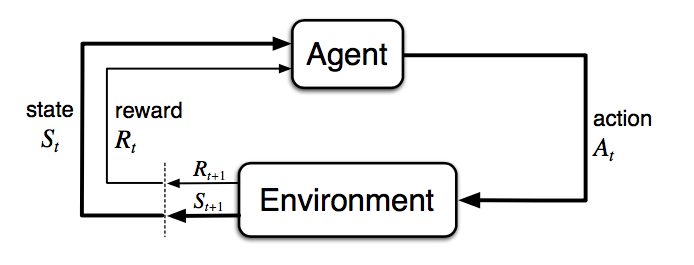
\includegraphics[scale=0.35]{mdp.png}
	\centering
	\caption{The agent-environment interaction in a Markov decision process\cite{n-step-return}.}
	\label{mdp}
\end{figure}

A Markov decision process consists of five elements $\mathcal{M} = \langle \mathcal{S}, \mathcal{A}, P, R, \gamma \rangle$, whose definition is shown in the following table:

\begin{center}
	\begin{tabular}{| p{0.12\linewidth} | p{0.27\linewidth} | p{0.45\linewidth} |}
		\hline
		\textbf{symbol} & \textbf{definition} & \textbf{function} \\
		\hline
		$\mathcal{S}$ & states of the agent &  \\ 
		\hline
		$\mathcal{A}$ & actions that the agent can choose &  \\ 
		\hline 
		$P$ & transition probability function & transition function:\newline $\mathcal{P}: \mathcal{S} \times \mathcal{A} \times \mathcal{S} \times \mathcal{R} \rightarrow \mathbb{R}_{\geq 0}$\newline state-transition function:\newline $\mathcal{P}: \mathcal{S} \times \mathcal{A} \times \mathcal{S} \rightarrow \mathbb{R}_{\geq 0}$\\
		\hline 
		$R$ & reward function & $\mathcal{R}: \mathcal{S} \times \mathcal{A} \rightarrow \mathbb{R}$ \\
		\hline 
		$\gamma$ & discounting factor for future rewards &  \\
		\hline 
	\end{tabular}
\end{center}

\par
Except for the notation of MDP, the reinforcement learning framework also consists of the following components:

\begin{center}
	\begin{tabular}{| p{0.12\linewidth} | p{0.27\linewidth} | p{0.45\linewidth} |}
		\hline
		\textbf{symbol} & \textbf{definition} & \textbf{function} \\
		\hline
		$\pi$ & policy function & deterministic:\newline $\pi: \mathcal{S} \rightarrow \mathcal{A}$ \newline stochastic:\newline $\pi: \mathcal{S} \times \mathcal{A} \rightarrow \mathbb{R}_{\geq 0}$\\ 
		\hline
		$G$ & return function & $G_{t} = \sum_{i=0}^{T}\gamma^i R_{i+t+1}$ \\ 
		\hline 
		$V_{\pi}$ & state value function & $V_{\pi}(s)=\mathbb{E}_{\pi}\left[G_{t} \mid S_{t}=s\right]$\\
		\hline 
		$Q_{\pi}$ & action-value function & $Q_{\pi}(s, a)=\mathbb{E}_{\pi}\left[G_{t} \mid S_{t}=s, A_{t}=a\right]$ \\
		\hline 
	\end{tabular}
\end{center}

\par
In the framework of meta-reinforcement learning, a reinforcement learning model is extended to Fig. \ref{meta-model}:

\begin{figure}[H]
	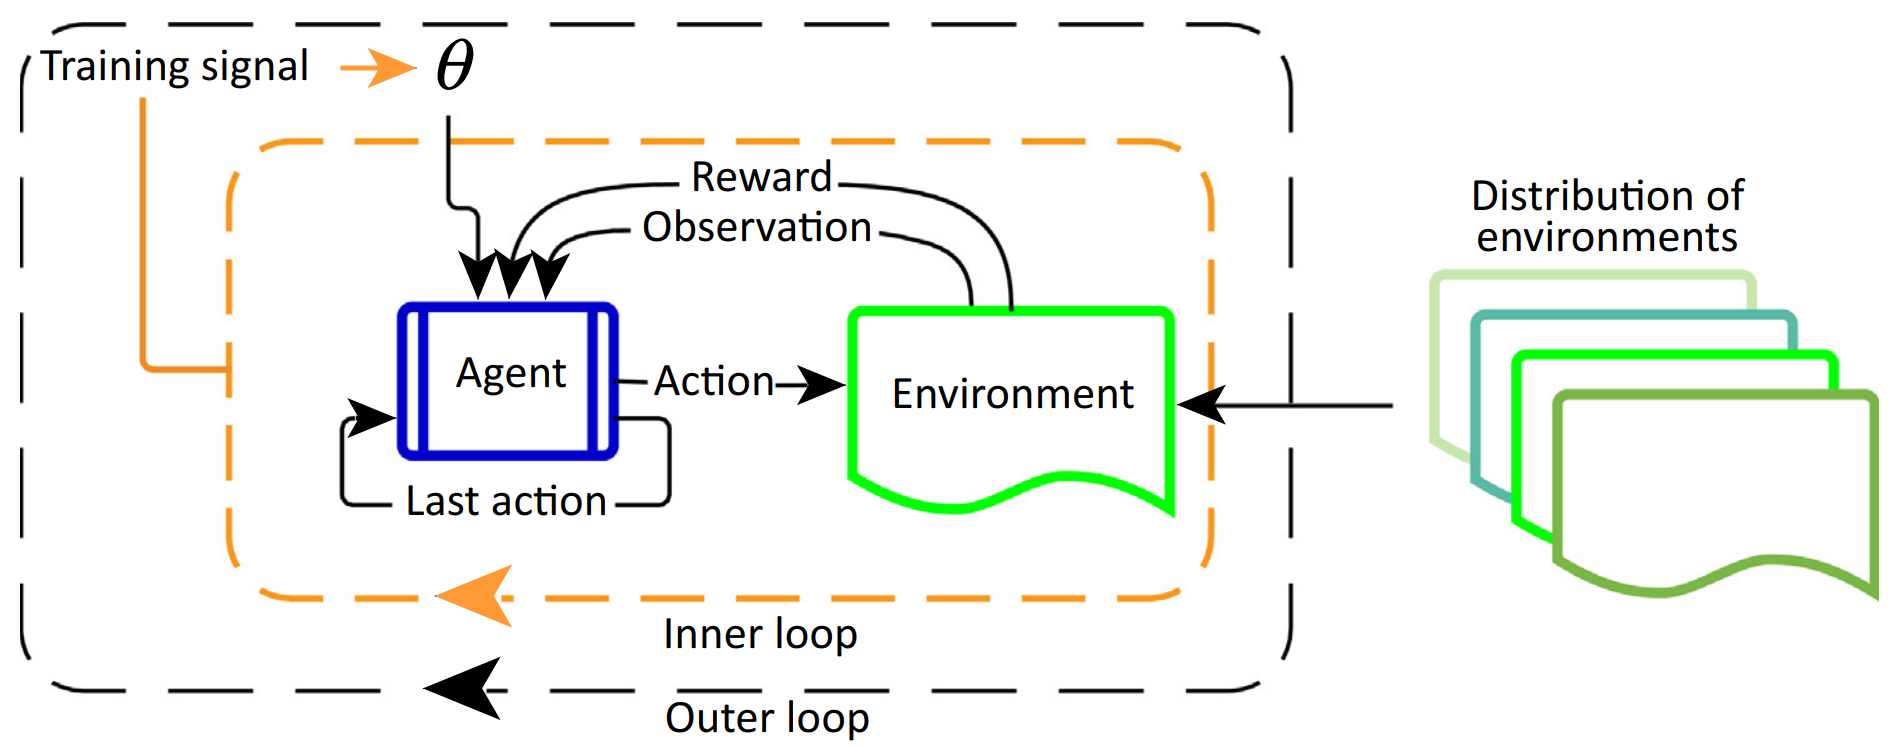
\includegraphics[scale=0.35]{meta-rl.png}
	\centering
	\caption{Schematic of meta-reinforcement Learning. The outer loop trains the parameter weights $\theta$, which determine the inner-loop learner ("Agent", instantiated by a recurrent neural network) that interacts with an environment for the duration of the episode. For every cycle of the outer loop, a new environment is sampled from a distribution of environments, which share some common structure\cite{meta-model}.}
	\label{meta-model}
\end{figure}

The agent is trained over specific learning tasks and optimized for the best performance in the inner loop, while in outer loop, the parameter of the learner is adjusted accordingly to yield the best performance on a distribution of tasks, including potentially unseen tasks.
	\section{Meta-Gradient Reinforcement Learning}
		One of the algorithm in meta reinforcement learning is the meta-gradient reinforcement learning introduced in \cite{meta-gradient} by Google DeepMind. The main idea of this algorithm is to update the meta-parameters $\eta$ to achieve a better learning performance. The details of this algorithm is presented in this section.

\par
In deep reinforcement learning, the environment model is often unknown to the agent. Therefore, the true value function has to be approximated by a function known as \textit{return} with parameter $\theta$. This return function plays an important role in determining the characteristics of the reinforcement learning algorithm. Usually, the return function is parameterised by a discount factor $\gamma$ and the bootstrapping parameter $\lambda$, which are denoted as meta-parameters $\eta$ in this paper. Throughout normal training process, these two parameters $\gamma$ and $\lambda$ are hand-selected and held fixed. Following are the \textit{n}-step return\cite{n-step-return} depending on fixed $\gamma$:

\[g_{\eta}\left(\tau_{t}\right)=R_{t+1}+\gamma R_{t+2}+\ldots,+\gamma^{n-1} R_{t+n}+\gamma^{n} v_{\theta}\left(S_{t+n}\right)\]

where $\eta = \{\gamma\}$, \textit{t} is the current time step, and the $\lambda$ return\cite{lambda-return} depending on fixed $\gamma$ and $\lambda$:

\[g_{\eta}\left(\tau_{t}\right)=R_{t+1}+\gamma(1-\lambda) v_{\theta}\left(S_{t+1}\right)+\gamma \lambda g_{\eta}\left(\tau_{t+1}\right)\]

where $\eta = \{\gamma, \lambda\}$. In addition, the parameter $\theta$ is updated by the following formula, taking fixed $\eta$ into account:

\[\theta' = \theta + f(\tau, \theta, \eta)\]

where $\tau$ is the sample of experience being considered.

\par
In order to achieve better performance, the algorithm introduced in \cite{meta-gradient} updates $\eta$ during the training process. Besides an objective function $J(\tau, \theta, \eta)$, whose value the parameter $\theta$ is being updated to reduce, a meta-objective defined as $\bar{J}\left(\tau^{\prime}, \theta^{\prime}, \bar{\eta}\right)$ is also included into this algorithm and the purpose of updating $\eta$ is to increase its value.

\par
Here is how the algorithm works: First, the algorithm starts with parameter $\theta$ and applies the update function on the first sample, resulting in an updated parameter $\theta'$. After that, the performance is measured by $\bar{J}(\tau', \theta', \bar{\eta})$, where $\tau'$ is the next sample following $\tau$ and $\bar{\eta}$ is a fixed meta-parameter. Then, the gradient of the meta-objective with respect to the meta-parameters $\eta$ is obtained by applying the chain rule:

\[\frac{\partial \bar{J}\left(\tau^{\prime}, \theta^{\prime}, \bar{\eta}\right)}{\partial \eta}=\frac{\partial \bar{J}\left(\tau^{\prime}, \theta^{\prime}, \bar{\eta}\right)}{\partial \theta^{\prime}} \frac{\mathrm{d} \theta^{\prime}}{\mathrm{d} \eta}\]

The term $\frac{\mathrm{d} \theta^{\prime}}{\mathrm{d} \eta}$ can be calculated as follows:

\begin{align*}
	\frac{\mathrm{d} \theta^{\prime}}{\mathrm{d} \eta}&=\frac{\mathrm{d} \theta}{\mathrm{d} \eta}+\frac{\partial f(\tau, \theta, \eta)}{\partial \eta}+\frac{\partial f(\tau, \theta, \eta)}{\partial \theta} \frac{\mathrm{d} \theta}{\mathrm{d} \eta} \\
	&=\left(\mathrm{I}+\frac{\partial f(\tau, \theta, \eta)}{\partial \theta}\right) \frac{\mathrm{d} \theta}{\mathrm{d} \eta}+\frac{\partial f(\tau, \theta, \eta)}{\partial \eta}
\end{align*}

In practice, the gradient $\partial f(\tau, \theta, \eta) / \partial \theta$ is large and challenging to compute, because it is a N x N matrix, where N is the number of parameters in $\theta$. Therefore, a simple approximation is to set $\partial f(\tau, \theta, \eta) / \partial \theta=0$, which is especially cheap to compute. Finally, $\Delta\eta$ is calculated as follows to maximize the meta-objective:

\[\Delta \eta = -\beta \frac{\partial \bar{J}(\tau', \theta', \bar{\eta})}{\partial \theta'} \frac{\partial f(\tau, \theta, \eta)}{d\eta}\]

where $\beta$ is the learning rate for updating $\eta$.

\par
The validation of meta-gradient algorithm is executed on Arcade Learning Environment with an agent built with the IMPALA framework. The agents are evaluated on 57 different Atari games and the median of human-normalised scores are documented in the following table:
\begin{figure}[H]
	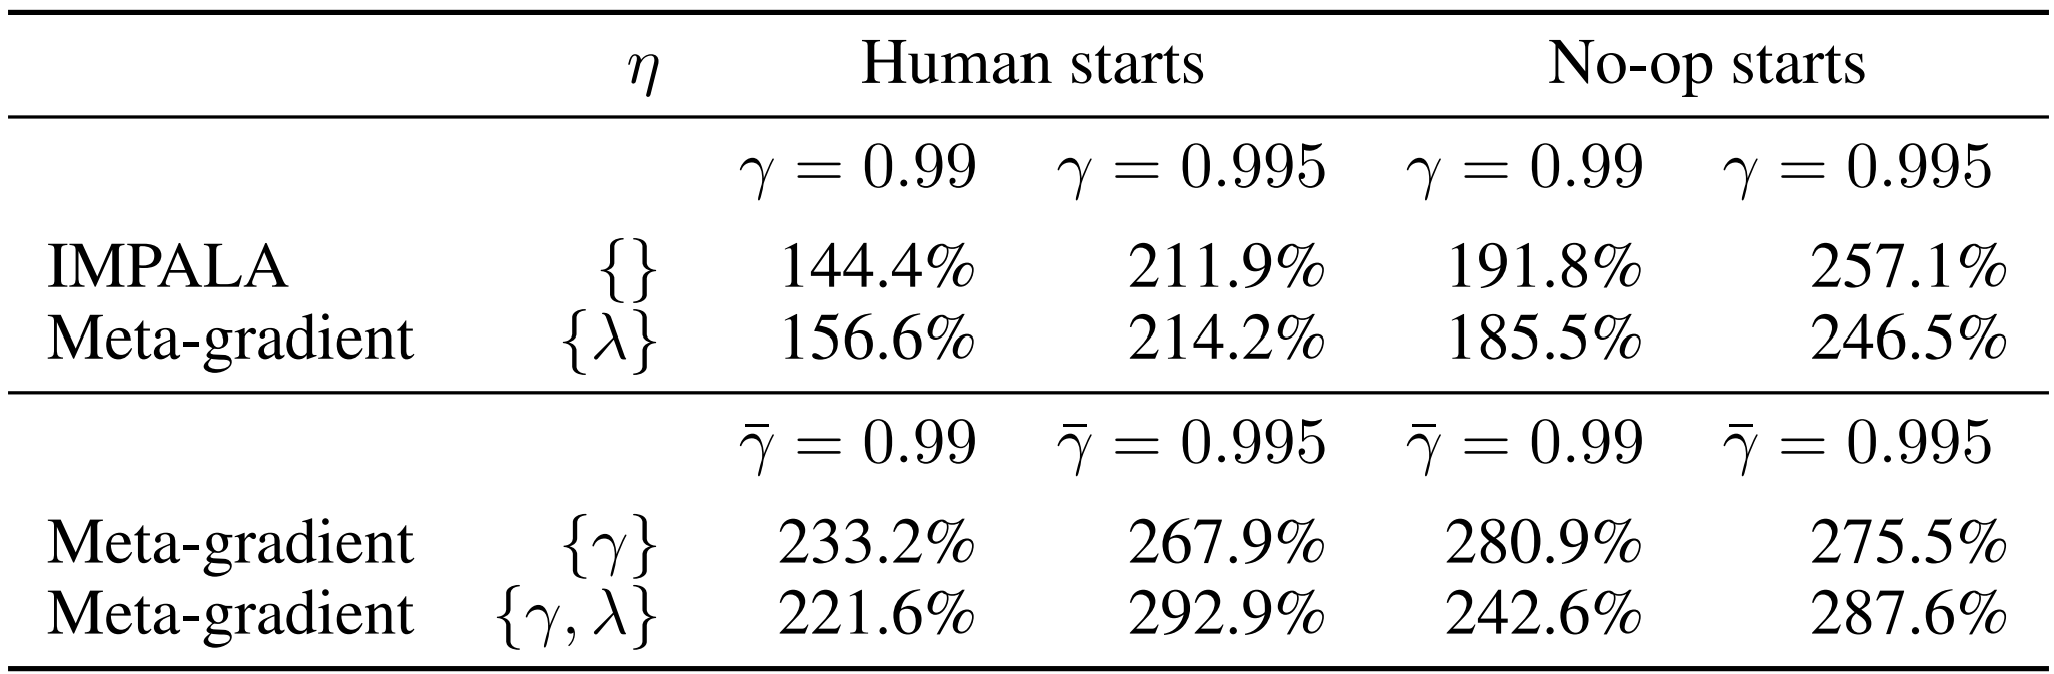
\includegraphics[scale=0.3]{meta-gradient-result.png}
	\centering
	\caption{Experiment result of meta-gradient algorithm. "Human starts" means episodes are initialized to a state that is randomly sampled from human play, while "No-op starts" means each episode is initialized with a random sequence of no-op actions.}
	\label{meta-gradient-result}
\end{figure}
We can see that meta-gradient algorithm has a better performance than the baseline IMPALA algorithm.
% 
% 
% 
	\section{Evolved Policy Gradient}
		Another algorithm for meta reinforcement learning is evolved policy gradient (EPG)\cite{epg}. Unlike meta gradient algorithm which focuses on learning the return function, EPG aims to learn a surrogate loss function $L_\phi = L_{\phi + \sigma\epsilon_i}$, which is parameterized by parameter $\phi$ along with a small Gaussian noise $\epsilon_i \sim \mathcal{N}(0, \mathbf{I})$ as perturbed terms.

\par
EPG contains an inner loop and an outer loop during its execution. In inner loop, the algorithm functions as normal policy gradient algorithm that tries to update policy parameter $\theta$ according to the following formula:

\[\theta^* = \argmin_\theta\EX_{\tau\thicksim\mathcal{M},\pi_\theta}[L_\phi(\pi_\theta,\tau)]\]

where $\theta^*$ is the updated parameter $\theta$, $\mathcal{M}$ is a sampled Markov decision process, $\tau$ is an episode of $\mathcal{M}$ with horizon $\textit{H}$. The objective of the inner loop is to minimize the loss function $L_\phi$. In outer loop, EPG adopts evolutionary strategies because there is no explicit way to write down a differentiable equation between the return and the loss function. The loss function parameter $\phi$ is updated as shown below:

\[\phi^* = \argmax_\phi\EX_{\mathcal{M}\thicksim p(\mathcal{M})}\EX_{\tau\thicksim\mathcal{M},\pi_{\theta^*}}[R_\tau]\]

where $p(\mathcal{M})$ is a distribution over MDPs, $\pi_{\theta^*}$ is the agent's policy trained with the loss function $L_\phi$ and $R_\tau = \sum_{t=0}^{H}\gamma^t{r_t}$ is the discounted episodic return of $\tau$. The goal of the outer loop is to achieve high expected returns in the MDP distribution.

\par
Pseudocode of EPG algorithm is shown in Fig. \ref{epg}:
\begin{figure}
	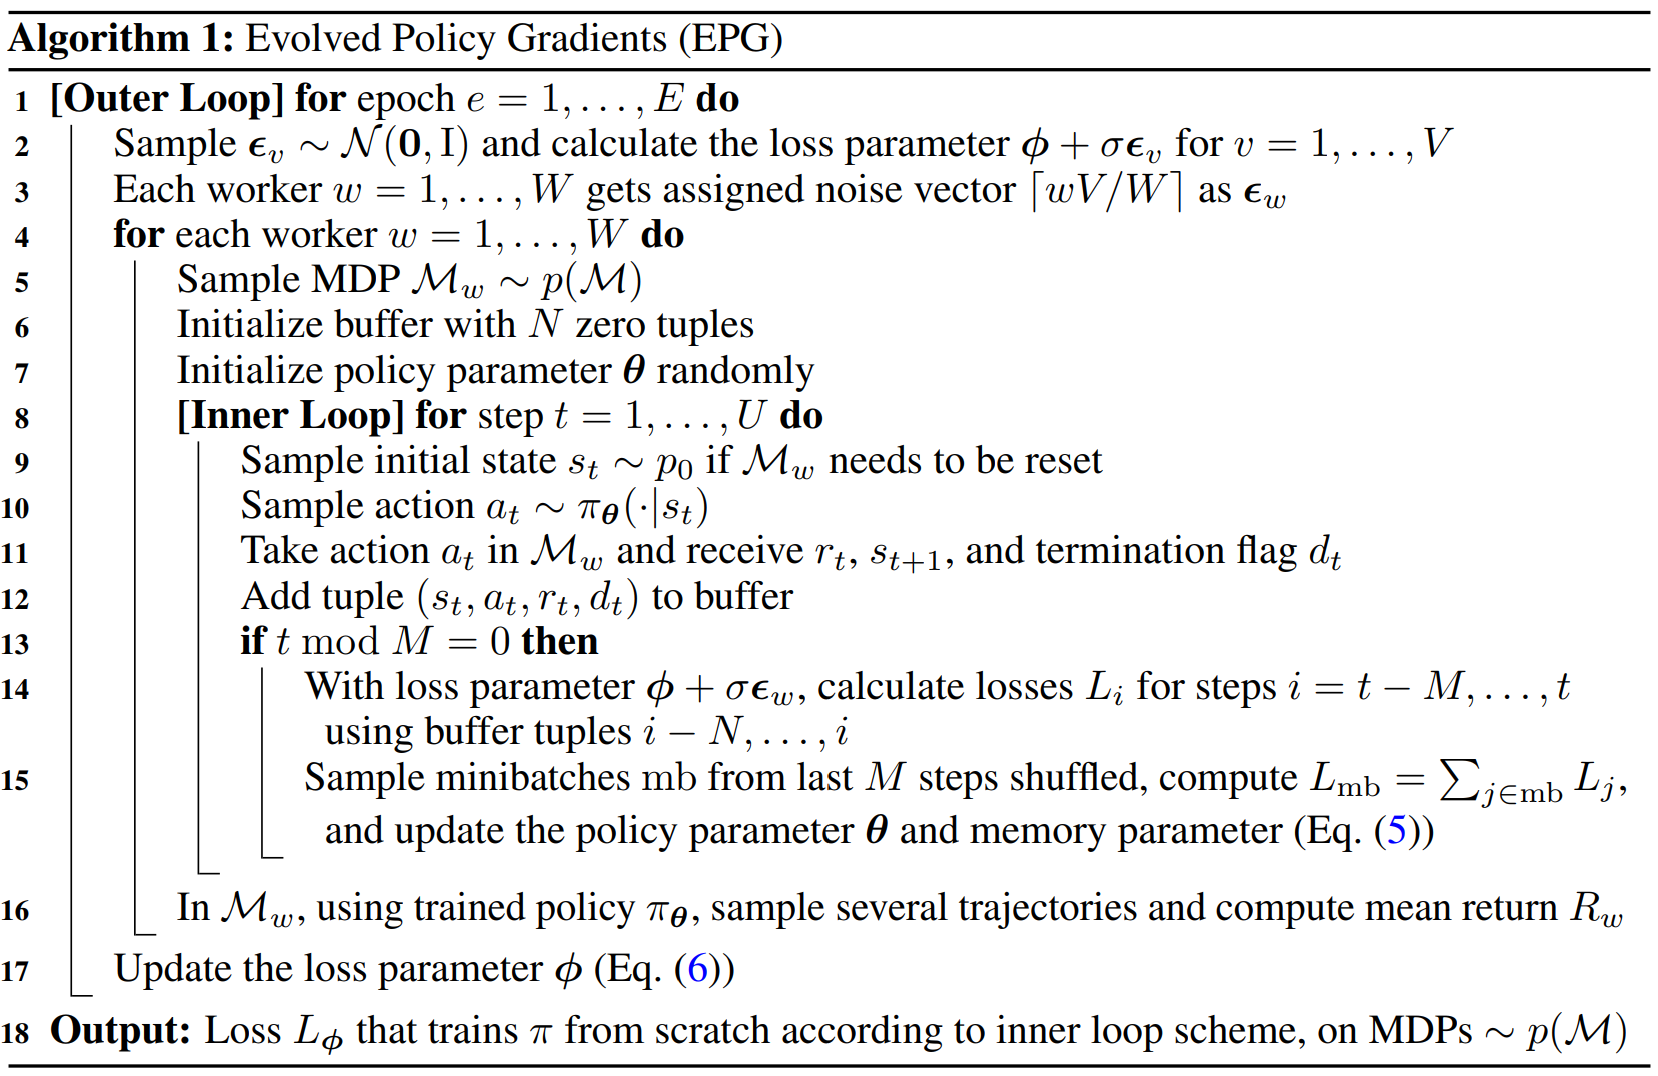
\includegraphics[scale=0.4]{epg.png}
	\centering
	\caption{EPG algorithm.}
	\label{epg}
\end{figure}

\par
The algorithm works as follows: Because of adoption of evolutionary strategies, $\textit{W}$ workers will work in the inner loop. Then, at the beginning of each epoch in the outer loop, $\textit{V}$ multivariate normal vectors $\epsilon_v \in \mathcal{N}(0,I)$ of the same dimension as the loss function parameter $\phi$ are generated and assigned to $\textit{V}$ loss functions $L_v = L_{\phi+\delta\epsilon_v}$ respectively, with $\textit{v}$ being the $\textit{v}$-th generated perturbed parameters. Then $\textit{W}$ workers are divided into $\textit{V}$ groups and each group obtain the $\textit{v}$-th loss function.

\par
Afterwards, the inner loop launches, each worker samples a random MDP from the task distribution $\mathcal{M}_\omega\thicksim p(\mathcal{M})$ and trains the policy $\pi_\theta$ along with the loss function $L_v$ given from the outer loop and updates the parameter $\theta$ with learning rate $\delta_{in}$ as follows:

\[\theta\gets\theta - \delta_{in}\cdot\nabla_\theta L_v(\pi_\theta,\tau_{t-M,...,t})\]

\par
At the end of the inner-loop training, the return $R_\omega$ is returned by each worker and is aggregated in the outer loop. Then, the parameter $\phi$ of the loss function is updated according to the rule shown below:

\[\phi\gets\phi+\delta_{out}\cdot\frac{1}{V_\sigma}\sum_{v=1}^{V}F(\phi+\sigma\epsilon_v)\epsilon_v\]

where $\delta_{out}$ is the learning rate and $F(\phi+\sigma\epsilon_v) = \frac{R_{(v-1)*W/V+1}+...+R_{v*W/V}}{W/V}$.

\par
The architecture of the loss function can be seen in Fig. \ref{loss-architecture}:
\begin{figure}
	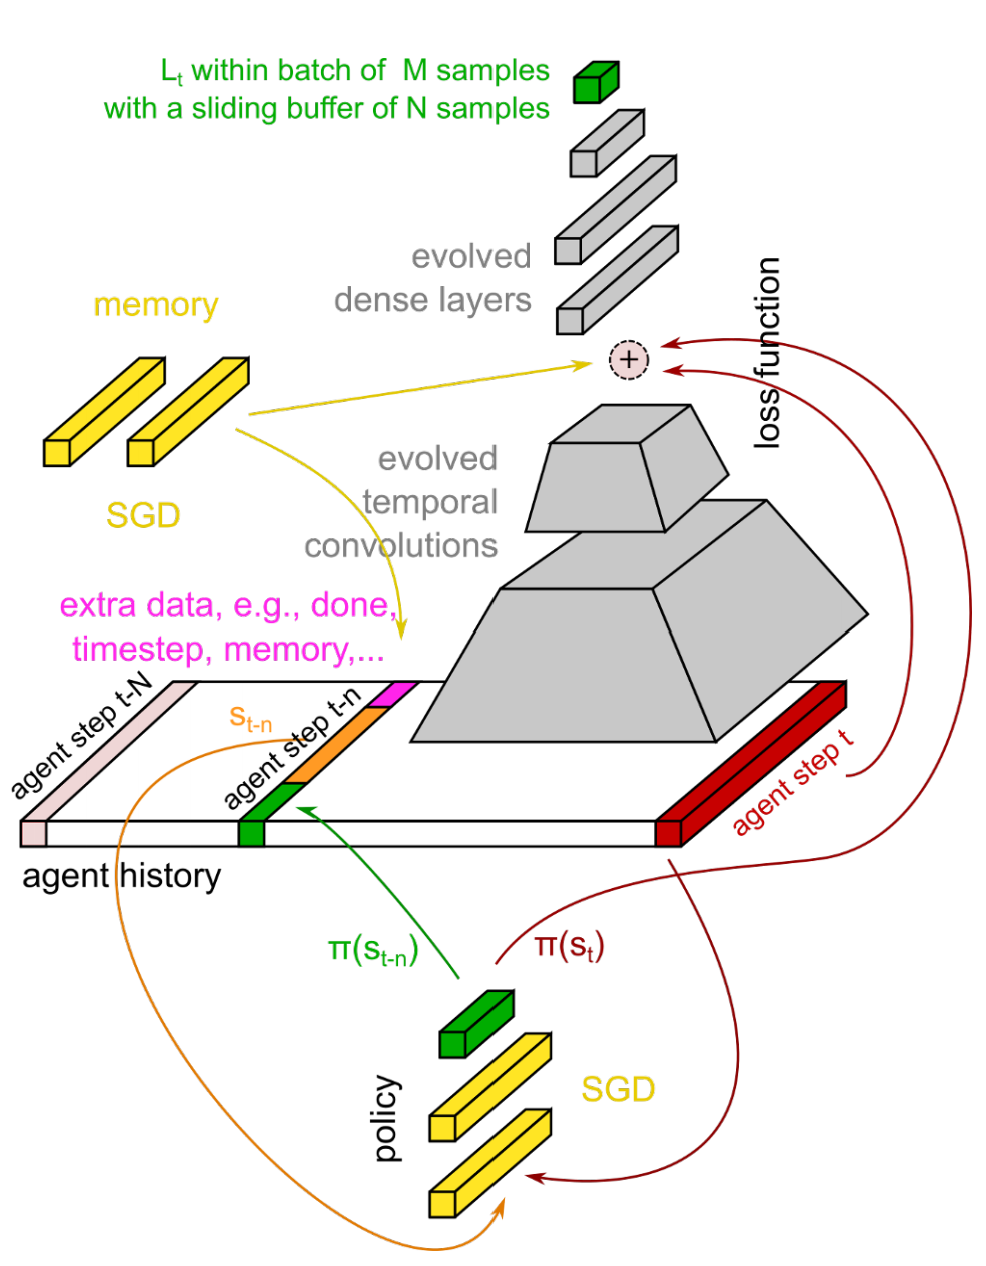
\includegraphics[scale=0.5]{loss-architecture.png}
	\centering
	\caption{Architecture of loss function $L_\phi$.}
	\label{loss-architecture}
\end{figure}

\par
As depicted in the diagram above, the architecture contains a memory unit, which is actually a single-layer neural network accepting constant input vector and is used to store the loss function value, as well as an experience buffer with limited storage, which stores the agent's \textit{N} most recent experience steps, in the form of a list of tuples $(s_t,a_t,r_t,d_t)$ at time step t, where \textit{$d_t$} is the trajectory termination flag.

\par
In addition, the architecture consists of temporal convolutional layers which generate a context vector $f_{context}$, and dense layers, which output the loss. The dense layer outputs the loss function \textit{$L_t$} at time step t by taking a batch of \textit{M} sequential samples $\{{s_i,a_i,d_i},mem,f_{context},\pi_\theta(\cdot|s_i)\}^t_{i=t-M}$. To generate the context vector, first, the data samples $\{{s_i,a_i,d_i},mem,\pi_\theta(\cdot|s_i)\}^t_{i=t-N}$ are stack together to form a matrix, second, this matrix is processed by the temporal convolutional layers which outputs the context vector $f_context$.

\par
This algorithm is evaluated under several randomized continuous control MuJoCo environments. Fig. \ref{hopper}, \ref{walker}, \ref{reacher} show the evaluation results on RandomHopper, RandomWalker and RandomReacher, which require the agent to identify a randomly sampled environment at test time via exploratory behavior. These diagrams show the learning curves of EPG and the off-the-shelf policy gradient method, PPO, under different settings. We can see that EPG agents learn more quickly and obtain higher returns compared to PPO agents.

\begin{figure}
	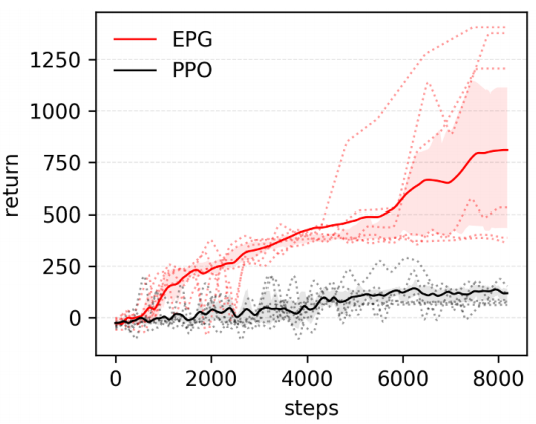
\includegraphics[scale=0.6]{hopper.png}
	\centering
	\caption{RandomHopper testtime training over 128 (policy updates) x64 (update frequency) = 8196 timesteps: PPO vs no-reward EPG.}
	\label{hopper}
\end{figure}
\begin{figure}
	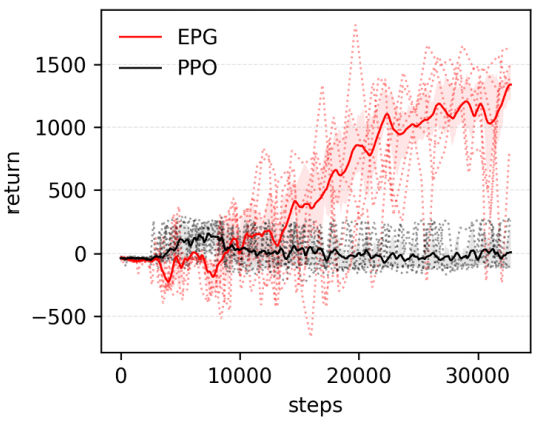
\includegraphics[scale=0.6]{walker.png}
	\centering
	\caption{RandomWalker testtime training over 256 (policy updates) x128 (update frequency) = 32768 timesteps: PPO vs no-reward EPG.}
	\label{walker}
\end{figure}
\begin{figure}
	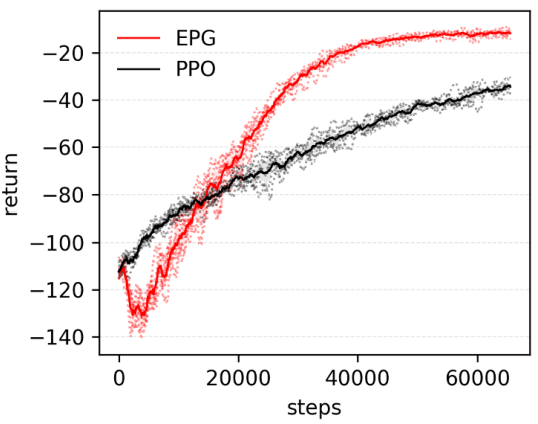
\includegraphics[scale=0.6]{reacher.png}
	\centering
	\caption{RandomReacher testtime training over 512 (policy updates) x128 (update frequency) = 65536 timesteps: PG vs no-reward EPG.}
	\label{reacher}
\end{figure}

\par
Fig. \ref{goal-ant}, \ref{metatrained-direction} and \ref{generalization-direction} show the ability of generalization of EPG. During metatraining, goals are randomly sampled on the positive x-axis (ant walking to the right) and at test time, goals are sampled from the negative x-axis (ant walking to the left). This task is illustrated in Fig. \ref{goal-ant}. Achieving generalization to the left side is not trivial, since it may be easy for a metalearner to overfit to the task metatraining distribution. As shown in Fig. \ref{metatrained-direction}, by training, $RL^2$ converges very fast, while EPG's performance catch up with $RL^2$ after 8192 steps. MAML achieves approximately the same final performance after taking a single SGD step (based on 8000 sampled steps).

\par
But when it comes to the generalization phase, as seen in Fig. \ref{generalization-direction}, the $RL^2$ and MAML algorithm are trapped by overfitting and yield negative result, while EPG trains the agent very quickly to the unseen task.
%We can see from these figures that EPG agents learn more quickly and obtain higher returns compared to PPO agents.

\begin{figure}
	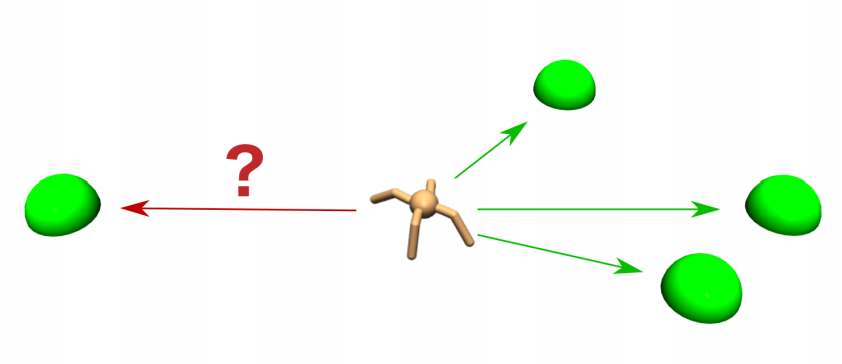
\includegraphics[scale=0.5]{goal-ant-task.png}
	\centering
	\caption{GoalAnt task illustration.}
	\label{goal-ant}
\end{figure}
\begin{figure}
	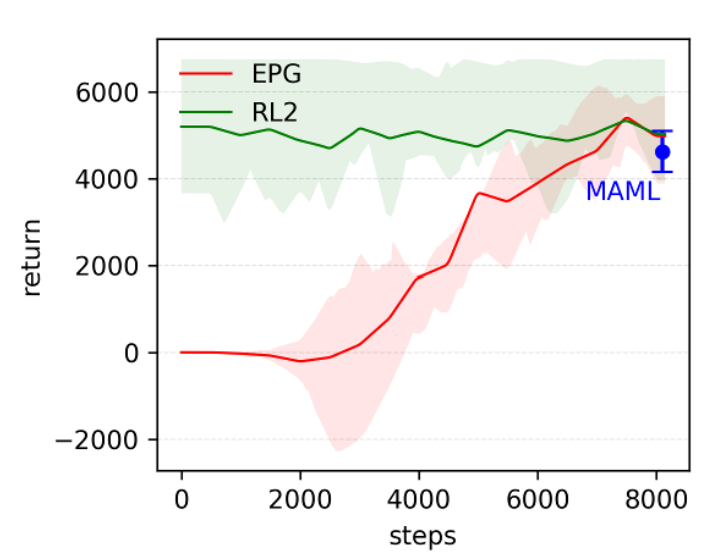
\includegraphics[scale=0.5]{metatrained-direction.png}
	\centering
	\caption{Metatrained direction.}
	\label{metatrained-direction}
\end{figure}
\begin{figure}
	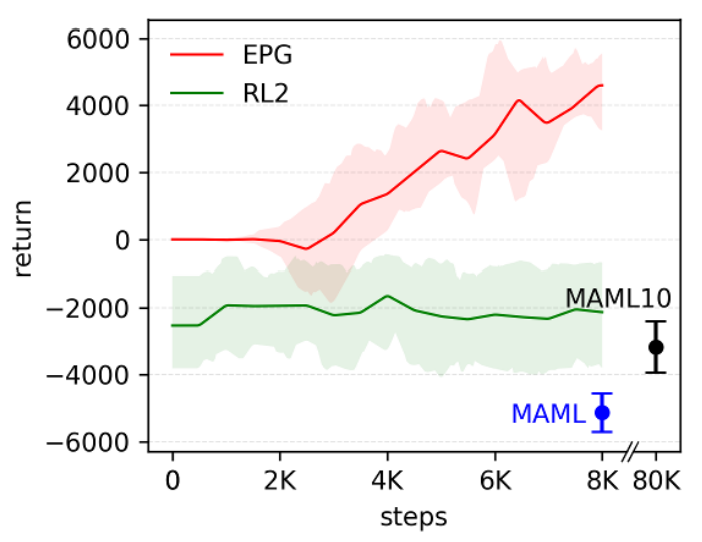
\includegraphics[scale=0.5]{generalization-direction.png}
	\centering
	\caption{Generalization direction.}
	\label{generalization-direction}
\end{figure}
	\section{MAML}
		% to do
	\section{MAESN}
		In this part, we introduce Model Agnostic Exploration with Structured Noise (MAESN) [8], by which an agent can be enabled to explore more effectively in new situations based on prior experience.
\subsection{overview}
 %As practical tasks are getting more and more complicated, the prior proposed exploration strategies, such as information gain [13] or state visitation bonuses [14], perform not as well as expected. The approach Model Agnostic Exploration with Structured Noise (MAESN), offers exploration strategies that are informed by prior knowledges and are more effective than random action-space noise.

The core idea of this gradient-based algorithm is to use prior experience both to initialize a policy and to learn a latent exploration space, by which the structured stochasticity injected policy can produce more effective exploration strategies on new tasks.

\subsection{ Meta-Learning Latent Variable Policies}
The conventional action distribution in reinforcement learning is written as $\pi_{\theta}(a \mid s)$, which possesses no property of temporally coherent randomness throughout the trajectory because it is independent for each time step. To address this problem we introduce latent variables $Z$. 
\begin{figure}[H]
	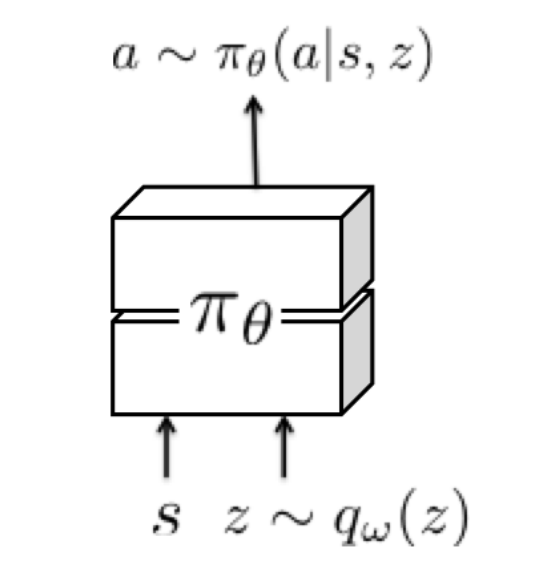
\includegraphics[scale=0.6]{MAESN_01.PNG}
	\centering
	\caption{latent variables}
	\label{MAESN}
\end{figure}

 We condition the policy on random variables, which are randomly drawn from a learned latent distribution. As the latent variable is sampled once per episode, the structured stochasticity in the process of exploration can be certainly ensured. The latent variable conditioned policy is represented as $\pi_{\theta}(a \mid s, z)$, where $z \sim q_{\omega}(z)$ and $q_{\omega}(z)$ is latent variable distribution with parameter $w$. 

Our aim is to meta-train the latent variable conditioned policy to generate coherent exploration strategies that perform faster adaptation on new tasks. Briefly, we jointly learn a set of policy parameters $\theta$ and the parameters of latent space distribution $w$, such that a policy gradient adaptation step can lead to maximal rewards.

\begin{figure}[H]
	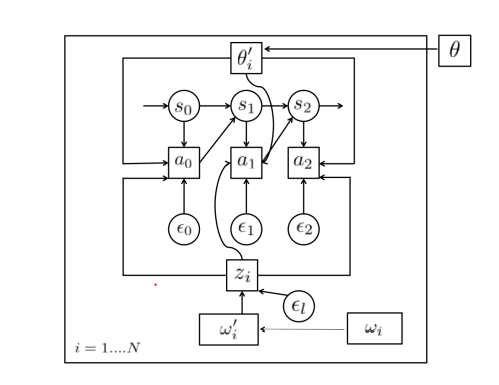
\includegraphics[scale=0.7]{MAESN_02.PNG}
	\centering
	\caption{Computation graph for MAESN}
	\label{MAESN}
\end{figure}

The objective of meta-training consists of not only sum of rewards under the post update parameters, but also the KL-divergence between the per-task pre-update distributions $q_{\omega_{i}}\left(z_{i}\right)$ and a prior $p(z)$, which ensures a effective structured exploration.
The full meta-training problem can be stated mathematically as:

\begin{figure}[H]
	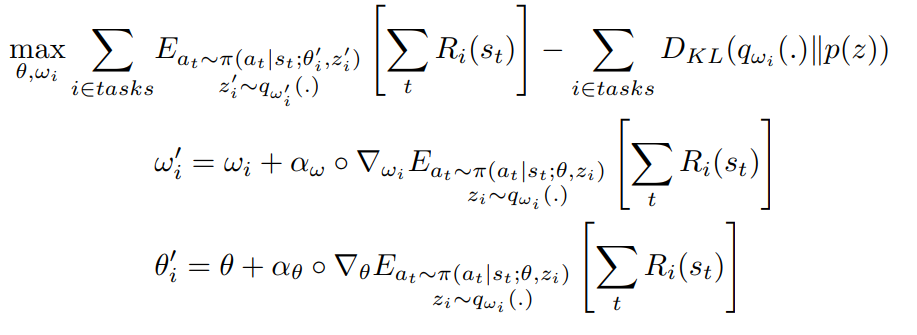
\includegraphics[scale=0.48]{MAESN_03.PNG}
	\centering
	\caption{meta-training procedure}
	\label{MAESN}
\end{figure}

The structure of training here is the same as the one in MAML, where two-level gradient is contained. The inner policy gradient is performed on the variational parameters for each task to get post-update parameters $\theta_{i}^{\prime}, \omega_{i}^{\prime}$, and then a meta-gradient is conducted to obtain $\theta$, $\omega_{0}$, $\omega_{1}$, ..., $\omega_{N}$.

\begin{figure}[H]
	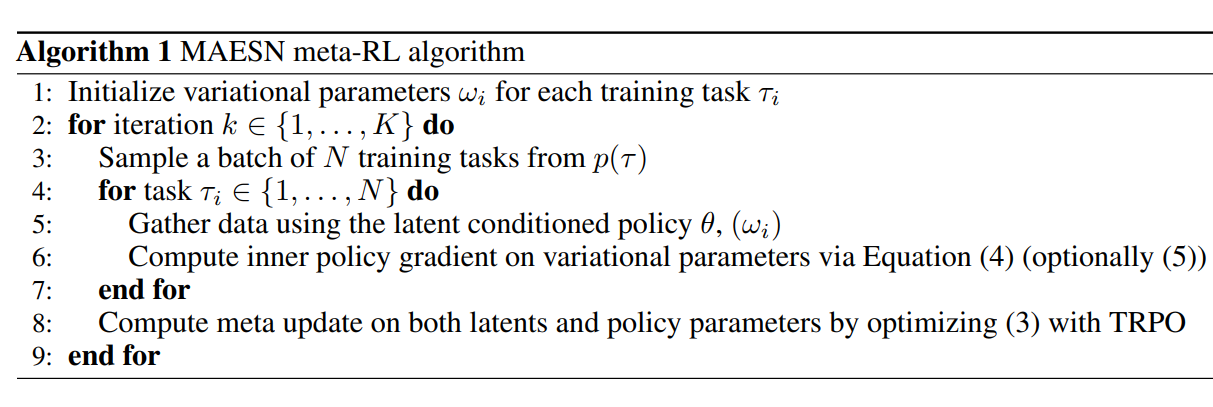
\includegraphics[scale=0.34]{MAESN_04.PNG}
	\centering
	\caption{MAESN algorithm}
	\label{MAESN}
\end{figure}

During the meta-train the sum of expected task rewards over all tasks is maximized and on the countrary the KL-divergence of pre-update distributions $q_{\omega_{i}}\left(z_{i}\right)$
against the prior$p\left(z_{i}\right)$ is minimized.
According to training procedure we can understand MAESN as augmentation of MAML with a latent space to inject structured noise.

Wenn adapting to new task, the variational parameters $\omega_{i}$ used during meta-training are not suitable anymore. $\omega$ is adapted by using the policy gradient via backpropagation on the RL objective:
$$
\max _{\omega} E_{a_{t} \sim \pi\left(a_{t} \mid s_{t}, \theta, z\right), z \sim q_{\omega}(.)}\left[\sum_{t} R\left(s_{t}\right)\right]
$$
In the inner loop, backpropagate through the sampling operation is needed to compute the gradients with respect to $\omega$, using either likelihood ratio or the reparameterization trick:

$$
\nabla_{\omega} \eta=E_{a_{t} \sim \pi\left(a_{t} \mid s_{t} ; \theta, z\right)}\left[\nabla \sim q_{\omega}(\cdot)^{ }\left[\nabla_{\omega} \log q_{\omega}(z) \sum_{t} R\left(s_{t}\right)\right]\right.
$$
With the introduction of latent variables we achieve a structured stochascity, which leads to time-correlated explorations. 

\subsection{Experiments and Evaluations}
In order to check the performance of meta-learned exploration strategies with MAESN, evaluations are conducted on three different task distributions with sparse rewards, which are Robotic Manipulation, Wheeled Locomotion and Legged Locomotion respectively. 

In Robotic Manipulation, a robotic hand is expected to push blocks to randomly chosen target locations, which is considered as a typical multi-manipulation skill for robot.
\begin{figure}[H]
	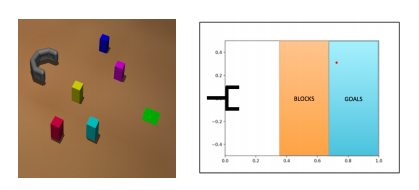
\includegraphics[scale=0.6]{MAESN_05.PNG}
	\centering
	\caption{Robotic Manipulation}
	\label{MAESN}
\end{figure}

In Wheeled Locomotion, a wheeled robot should move to different randomized goal locations with coherent exploration strategies.
\begin{figure}[H]
	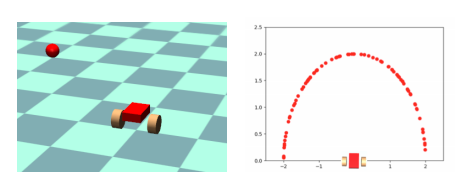
\includegraphics[scale=0.53]{MAESN_06.PNG}
	\centering
	\caption{Wheeled Locomotion}
	\label{MAESN}
\end{figure}

In Legged Locomotion, an ant walks to randomly placed goals, which requires carefully coordinated leg motions.
\begin{figure}[H]
	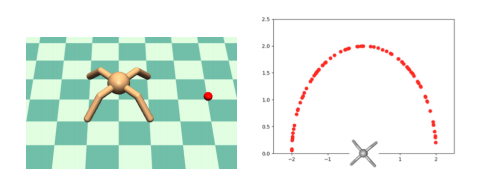
\includegraphics[scale=0.53]{MAESN_07.PNG}
	\centering
	\caption{Legged Locomotion}
	\label{MAESN}
\end{figure}
In the same time we compare MAESN with other 6 exploration approaches during meta-test on each task distribution, that are RL$^2$, MAML, simply learning latent spaces without fast adaptation(LatentSpace), TRPO, REINFORCE, and training from scratch with VIME. 

\begin{figure}[H]
	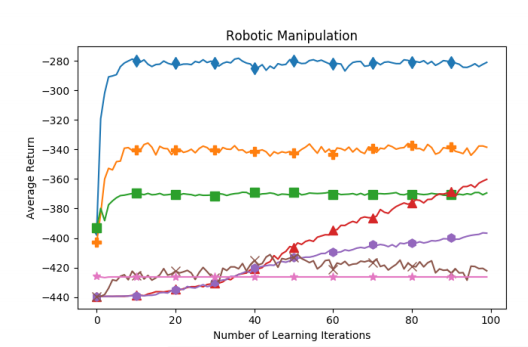
\includegraphics[scale=0.6]{MAESN_09.PNG}
	\centering
	\caption{results of Robotic Manipulation}
	\label{MAESN}
\end{figure}
\begin{figure}[H]
	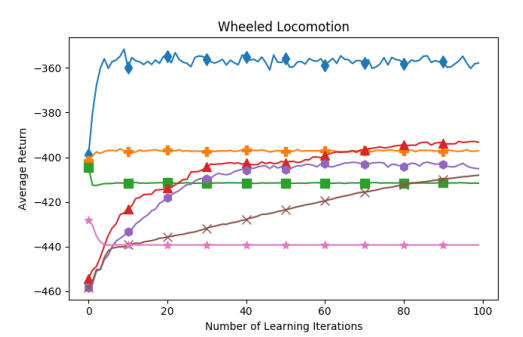
\includegraphics[scale=0.6]{MAESN_10.PNG}
	\centering
	\caption{results of Wheeled Locomotion}
	\label{MAESN}
\end{figure}
\begin{figure}[H]
	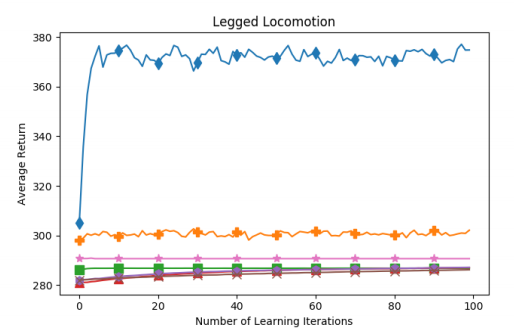
\includegraphics[scale=0.6]{MAESN_11.PNG}
	\centering
	\caption{results of Legged Locomotion}
	\label{MAESN}
\end{figure}
From the results of all exploration strategies we find that the latent variable based MAESN performs much better on new tasks compared to either prior meta-learning approaches or the methods learning from scratch, since MAESN is able to train latent space for fast adaptation.










	
	
	\section{Conclusion}
	In this article we took a research on meta reinforcement learning, by which meta-learning is performed in the field of reinforcement learning. The aim is to help optimize the model to solve unseen tasks in the minimum amount of time. We analysed four gradient-based algorithms of meta reinforcement learning, which are Meta-Gradient Reinforcement Learning, Evolved Policy Gradient, MAML and MAESN respectively.
	
	%The key point of Meta-Gradient Reinforcement Learning is to achieve a better learning performance by updating the meta-parameters $\eta$. And Evolved Policy Gradients is the method that evolves the loss function of learning agents, which can enable fast training on novel tasks.这块我大概写了一些,不是太了解,你可以修改一下
	
	As an essential meta-learning approach, Model-Agnostic Meta-Learning (MAML) can enable an agent to quickly acquire a policy for a new test task using only a small amount of experience. On the one hand it is model agnostic, on the other hand it can be combined with any model representation
    that is optimized by gradient descent.
    
    Additionally, Model Agnostic Exploration with Structured Noise (MAESN) is a combination of structured stochasticity and MAML. The advantage lies in that with the help of latent space, that injects coherent stochasticity into the policy, MAESN is able to provide a structured exploration behavior and to achieve fast adaptation on new task during meta-test time.
	
	
	
	
	% conference papers do not normally have an appendix
	
	
	% use section* for acknowledgment
	\section*{Acknowledgment}
	
	
	The authors would like to thank...
	
	
	
	
	
	% trigger a \newpage just before the given reference
	% number - used to balance the columns on the last page
	% adjust value as needed - may need to be readjusted if
	% the document is modified later
	%\IEEEtriggeratref{8}
	% The "triggered" command can be changed if desired:
	%\IEEEtriggercmd{\enlargethispage{-5in}}
	
	% references section
	
	% can use a bibliography generated by BibTeX as a .bbl file
	% BibTeX documentation can be easily obtained at:
	% http://mirror.ctan.org/biblio/bibtex/contrib/doc/
	% The IEEEtran BibTeX style support page is at:
	% http://www.michaelshell.org/tex/ieeetran/bibtex/
	%\bibliographystyle{IEEEtran}
	% argument is your BibTeX string definitions and bibliography database(s)
	%\bibliography{IEEEabrv,../bib/paper}
	%
	% <OR> manually copy in the resultant .bbl file
	% set second argument of \begin to the number of references
	% (used to reserve space for the reference number labels box)
	\begin{thebibliography}{1}
		
		%\bibitem{IEEEhowto:kopka}
		%H.~Kopka and P.~W. Daly, \emph{A Guide to \LaTeX}, 3rd~ed.\hskip 1em plus
		%0.5em minus 0.4em\relax Harlow, England: Addison-Wesley, 1999.
		
		
		\bibitem{n-step-return}
		R. S. Sutton and A. G. Barto., \emph{Reinforcement learning: An introduction}.
		
		\bibitem{meta-model}
		Matthew Botvinick, Sam Ritter, Jane X. Wang, Zeb Kurth-Nelson, Charles Blundell, and
		Demis Hassabis, \emph{Reinforcement Learning, Fast and Slow}.
		\url{URL: https://www.cell.com/action/showPdf?pii=S1364-6613%2819%2930061-0}
		
		\bibitem{meta-gradient}
		Zhongwen Xu, Hado van Hasselt and David Silver, \emph{Meta-Gradient Reinforcement Learning}.
		\url{URL: https://proceedings.neurips.cc/paper/2018/file/2715518c875999308842e3455eda2fe3-Paper.pdf}
		
		\bibitem{lambda-return}
		R. S. Sutton, \emph{Learning to predict by the methods of temporal differences}.
		
		\bibitem{epg}
		Rein Houthooft, Richard Y. Chen, Phillip Isola, Bradly C. Stadie, Filip Wolski, Jonathan Ho, Pieter Abbeel, \emph{Evolved Policy Gradients}.
		\url{URL: https://papers.nips.cc/paper/2018/file/7876acb66640bad41f1e1371ef30c180-Paper.pdf}
		
		\bibitem{MAML}
		Chelsea Finn, Pieter Abbee, Sergey Levine, \emph{Model-Agnostic Meta-Learning for Fast Adaptation of Deep Networks}.
		\url{https://arxiv.org/pdf/1703.03400.pdf}
		
		\bibitem{MAML}
		Marcin Andrychowicz, Misha Denil,  Sergio Gómez Colmenarejo, Matthew W. Hoffman, David Pfau, Tom Schau, Brendan Shillingford,
		Nando de Freitas, \emph{Learning to learn by gradient descent
by gradient descent}.
		\url{https://arxiv.org/pdf/1606.04474.pdf}
		
		\bibitem{MAML}
		Ravi, Sachin and Larochelle, Hugo, \emph{Optimization as a model for few-shot learning}.
		\url{https://openreview.net/pdf?id=rJY0-Kcll}
		
		\bibitem{MAML_Experiment}
		Williams, Ronald J, \emph{Simple statistical gradient-following
        algorithms for connectionist reinforcement learning}.
		\url{}
		
		\bibitem{MAML_Experiment}
		John Schulman, Sergey Levine, Philipp Moritz, Michael I. Jordan, Pieter Abbeel, \emph{Trust Region Policy Optimization}.
		\url{https://arxiv.org/abs/1502.05477}
		
		\bibitem{MAML_Experiment}
		Todorov, Emanuel, Erez, Tom, and Tassa, Yuval, \emph{MuJoCo: A physics engine for model-based control}.
		\url{https://ieeexplore.ieee.org/document/6386109}
		
		\bibitem{MAESN}
		Abhishek Gupta, Russell Mendonca, YuXuan Liu, Pieter Abbeel, Sergey Levine, \emph{Meta-Reinforcement Learning of Structured Exploration Strategies}.
		\url{https://arxiv.org/abs/1802.07245}
		
		\bibitem{MAESN}
		Daniel Russo, Benjamin Van Roy, \emph{Learning to Optimize via Information-Directed Sampling}.
		\url{https://arxiv.org/abs/1403.5556}
		
		\bibitem{MAESN}
		Zhi-Xiong Xu, Xi-Liang Chen, Lei Cao, Chen-Xi Li, \emph{A study of count-based exploration and bonus for reinforcement learning}.
		\url{https://ieeexplore.ieee.org/document/7951951}
		
		\bibitem{MAESN_experiment}
		Y. Duan, J. Schulman, X. Chen, P. L. Bartlett, I. Sutskever, and P. Abbeel, \emph{RL$^2$: Fast reinforcement learning via slow reinforcement learning}.
		\url{https://ieeexplore.ieee.org/document/7951951}
		
		\bibitem{MAESN_Evaluation}
		Rein Houthooft, Xi Chen, Yan Duan, John Schulman, Filip De Turck, Pieter Abbeel, \emph{VIME: Variational Information Maximizing Exploration}.
		\url{https://arxiv.org/abs/1605.09674}
		
	\end{thebibliography}
	
	
	
	
	% that's all folks
\end{document}